

\section{Event Driven Programming}


In ``batch programming'', as the name suggests, a group of instructions is executed regardless of the physical situation and the events occurring during the simulations. As opposed to this, in an event driven program the simulation depends on what is actually happening in the simulated system\footnote{Note that this is not completely true, since it can also be the case for some particular routines based on batch programming, e.g. for adaptive time steps. This statement has to be taken as a loose classification of various programming philosophies rather than a strict rule.}. The flow is therefore interrupted by branching points and is ruled by conditional logic. These kinds of programs are generally difficult to parallelize due to their unpredictable nature. ``Unpredictable'', in the sense that the computations that the program executes strongly depend on the starting conditions of the problem and the evolution of the system. This is the reason why they typically are unpredictable. These general statement will become clearer with some concrete and intuitive examples.


\subsection{Elastic Collisions}

One of the first examples for event driven programming applied to molecular dynamics can be found in a publication by Alder  \citep{alder_spheres}. He considered rigid bodies of finite volume (like a set of billiard balls) which can be mathematically modeled by a hard core potential. This cannot be handled with the MD methods we learned, since the derivative of the potential diverges. In his simulation, Alder regarded the collisions between particles as instantaneous events without any further interaction between the particles but the collisions. This way, one can avoid the calculation of the forces, and only treat the momentum exchange during the collision. Mind that three body problems are neglected in the continuum mechanics of hard spheres and the calculations can therefore be solved analytically in some cases. We will start by describing the simplest of all cases: friction-free interaction of spheres with uniform density distribution.

Assuming that the collisions are instantaneous events with no influence on the dynamics before and after the impact, the system evolves undisturbed during the time in which no collision happens, $t_c$. The calculation of the uniform motion of the particles is relatively inexpensive, as it is the elastic collision of the particles involved in the impact. The expensive part of the program is the calculation of the time when the next collision occurs, since one has to go through all pairs of particles.

\vspace{0.1cm}
\noindent
\begin{minipage}{\textwidth}
\begin{minipage}{.001\textwidth}
 \end{minipage}\hfill
\begin{minipage}{.99\textwidth}
  \centering
  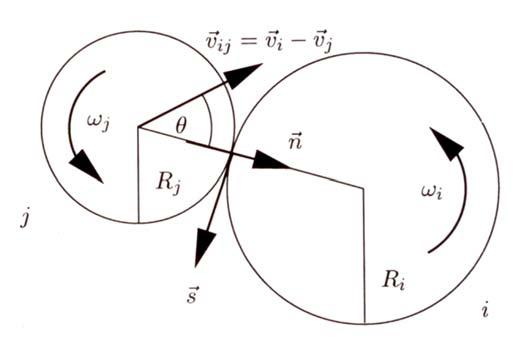
\includegraphics[width=.85\textwidth]{pics/2Dcollision}
  \captionof{figure}{Parameters for the collision event of two elastic disks.}
  \label{fig:2Dcollision}
\end{minipage}
\end{minipage}
\vspace{0.1cm}

In 2D, we can consider the collision of two disks $i$ and $j$. The \emph{collision angle} is defined as the angle betwee the connecting vector $\vec{r}_{i,j} \equiv \vec{r}_i-\vec{r}_j$ and the relative velocity $\vec{v}_{i,j} \equiv \vec{v}_i-\vec{v}_j$ (see Fig. \ref{fig:2Dcollision}). For the beginning, we will neglect the rotation since we are in a frictionless regime. The time $t_{i,j}$ at which the next collision between the particle $i$ and the particle $j$ would occur can be calculated using the formulae of uniform motion. From the vector connecting the centers of the particles
\begin{equation}
\abs{\vec{r}_{i,j}} \equiv \vec{r}_j-\vec{r}_i
\end{equation}
we can impose a certain length ($ \abs{R}_j+\abs{R}_i$) at the contact time and from their relative velocity ${v}_{i,j}$, the contact time of two particles can be calculated by solving 
\begin{equation}
{v}_{i,j}^2{t}_{i,j}^2 + 2\kl{\vec{r}_{i,j}^0 \vec{v}_{i,j}^2}{t}_{i,j} + \kl{{r}_{i,j}^0}^2 -\kl{ \vec{R}_i+\vec{R}_j}^2=0.
\label{eq:first_contact} 
\end{equation}
Mind that \eqref{eq:first_contact} only has valid solutions if the trajectories of the particles $i$ and $j$ do cross. The time $t_c$ when the next collision occurs in the system is then the minimum over all pairs $i,j$:

\begin{equation}
t_c=\underset{i,j}{\text{min}}\ekl{t_{i,j}}
\end{equation}

It is also possible to add simple external forces like the one induced by a gravitational or electromagnetic field. The main issue with this method is that the loop is very time consuming since it is of order $N^2$. For every step, one has to go through two minimization problems: first one has to find for each particle $i$ which will be the first particle $j$ that will collide with $i$ and calculate the collision time $t_{i,j}$.  If the system is very densely packed, there is no need to do the calculations for particle that are separated by large distances (large relatively to their mean free path). For this, the knowledge of the distance between each pair of particles is needed and the calculation would be very expensive. Instead of looking at the distances between particles one can divide the system into sectors and treat the sectors separately. The crossing of the particles through the sector boundaries has to be treated as a collision.
A further way of acelerating the algorithm is given by the \emph{Lubachevsky method}.




\subsection{Lubachevsky method}

Instead of going through all the pairs, one can create a list of events for each particle. In the list the events are stored keeping record of the time and particles involved in the previous and in the next  collision. After that an the particles are ordered depending on their next collision time. There will always be two particles for every collision time. When the collision occurs one has to reorganize  the system and the list of events only for the new particle. The reordering of the event list takes a time in the order of $O\kl{\text{log}N}$. The advantages of this method are that it is not necessary to minimize all the collision times of all the pairs at every step, and that it is unnecessary to propagate the particles that will not collide. Only the position and velocity of the particle involved in the event have to be updated. The rearrangement of the event list can be done via tournament trees instead of going through all the particles.



\subsubsection*{Collision with perfect slip:}

In a first approximation we will neglect that the particles can also exchange momentum tangentially. Angular momentum is therefore irrelevant, and only linear momentum is exchanged. We can use momentum 

\begin{align}
{\vec{v}_i}^{\,\text{after}} &= {\vec{v}_{i}}^{\,\text{before}} + \frac{\vec{\Delta p}}{m_i} \\
{\vec{v}_j}^{\,\text{after}} &= {\vec{v}_{j}}^{\,\text{before}} - \frac{\vec{\Delta p}}{m_j}
\end{align}
and energy conservation
\begin{equation}
\frac{1}{2}m_i \kl{\vec{v}_i^{\,\text{before}}}^2 + \frac{1}{2}m_j \kl{\vec{v}_j^{\,\text{before}}}^2 
=
\frac{1}{2}m_i \kl{\vec{v}_i^{\,\text{after}}}^2 + \frac{1}{2}m_j \kl{\vec{v}_j^{\,\text{after}}}^2 
\end{equation}
and we obtain the exchanged momentum: 
\begin{equation}
\vec{\Delta p} = -2 m_{\text{eff}} \ekl{\kl{\vec{v}_i^{\,\text{before}}-\vec{v}_j^{\,\text{before}}}\cdot\vec{n}}\vec{n}
\end{equation}
with $m_{eff}=\frac{m_i m_j}{m_i+m_j}$ being the \emph{effective mass}. If $m_i=m_j$ the collision event boils down to the simple relation
\begin{align}
{\vec{v}_i}^{\,\text{after}} &= {\vec{v}_{i}}^{\,\text{before}} - {\vec{v}_{ij}}^{\,n}\cdot\vec{n} \\
{\vec{v}_j}^{\,\text{after}} &= {\vec{v}_{j}}^{\,\text{before}} + {\vec{v}_{ij}}^{\,n}\cdot\vec{n}
\end{align}
The values can be stored once in a look-up table such that there is no need of calculating the correction to the velocities at every collision.








\subsubsection*{Collision with rotation:}

If particles collide with a nonzero tangengial velocity they can exchange angular momentum due to friction. This, together with linear and angular momentum conservation has to be taken into account. As known from classical physics, the equation of motion for rotations holds:


\begin{equation}
I\der{\vec{\omega}_i}{t} = \vec{r}\times\vec{f}_{i,j} = m\vec{r}\times\der{\vec{v}_i}{t},
\end{equation}
with the moment of inertia $I$. If we consider the collision between spheres having the same radius $R$, moment of inertia $I$ and mass $m$ the exchange of angular momentum is given by

\begin{align*}
I\kl{\vec{\omega}_i\,'-\vec{\omega}_i} &= -R m \kl{\vec{v}_i\,'-\vec{v}_i}\times\vec{n}\\
I\kl{\vec{\omega}_j\,'-\vec{\omega}_j} &=  R m \kl{\vec{v}_j\,'-\vec{v}_j}\times\vec{n}
\end{align*}
with the primed velocities being the ones after the collision. Together with the conservation of linear momentum

\begin{equation*}
\vec{v}_i'+\vec{v}_j\,' = \vec{v}_i+\vec{v}_j,
\end{equation*}

one obtains the rule for calculating the new angular velocity after the collision: 

\begin{equation}
\vec{\omega}_i\,'-\vec{\omega}_i = \vec{\omega}_j\,'-\vec{\omega}_j = \frac{R m}{I} \kl{\vec{\vec{v}}_i\,'-\vec{\vec{v}}_i} \times \vec{n}
\label{eq:ang_vel_diff}
\end{equation}

We can decompose the relative velocity $\vec{u}$ of the particles into normal ($\vec{u}^{\,n}$) and tangential ($\vec{u}^{\,t}$) velocity. Mind that we are not interested in the relative velocities of the centers of mass of the particles. What is important for the transfer of angular momentum is the relative velocity of the particles' surfaces at the contact point.
 
\begin{align*}
\vec{u}_{i,j}^{\,n} &= \kl{\vec{u}_{i,j} \vec{n}} \vec{n}  \\
\vec{u}_{i,j}^{\,t} &= \vec{u}_{i,j} \times \vec{n} = \ekl{\kl{\vec{v}_{i}-\vec{v}_{j}} - R\kl{\vec{\omega}_{i}+\vec{\omega}_{j}}}\times\vec{n}
\end{align*}

We can now introduce an artificial parameter that describes the general slip condition:

\begin{equation}
\vec{u}_{i,j}^{\,t}\,' = e_t \vec{u}_{i,j}^{\,t} 
\label{eq:slipc}
\end{equation}


The perfect slip collision is recovered by setting  $e_t=1$, which means that no rotation energy is transferred from one particle to the other, or the extreme case in which there is no slip at all: $e_t=0$. Energy conservation of the system holds only if $e_t=1$, for $ e_t<1$ energy is dissipated. In case of negative coefficient we speak of \emph{superelasticity}.

If we compute the difference of the relative tangential velocities before and after the slip we get

\begin{align*}
\vec{u}_{i,j}^{\,t}-\vec{u}_{i,j}^{\,t}\,' 
&=
\ekl{\kl{\vec{v}_{i}-\vec{v}_{j}} - R\kl{\vec{\omega}_{i}+\vec{\omega}_{j}}}\times\vec{n}
-
\ekl{\kl{\vec{v}_{i}'-\vec{v}_{j}'} - R\kl{\vec{\omega}_{i}'+\vec{\omega}_{j}'}}\times\vec{n}\\
&=
\ekl{\kl{\vec{v}_{i}'-\vec{v}_{i}-\vec{v}_{j}'+\vec{v}_{j}} - R\kl{\vec{\omega}_{i}'-\vec{\omega}_{i} + \vec{\omega}_{j}'-\vec{\omega}_{j}  }}\times\vec{n}\\
\end{align*}
And using \eqref{eq:ang_vel_diff} we get an expression without angular velocities:

\begin{align*}
\vec{u}_{i,j}^{\,t}-\vec{u}_{i,j}^{\,t}\,' 
&=
\kl{1-e_t}\vec{u}_{i,j}^{\,t} \\
&=-\ekl{2\kl{\vec{v}_{i}'-\vec{v}_{i}} + 2q \kl{\vec{v}_{i}'-\vec{v}_{i}} }\times\vec{n}
\end{align*}
\vspace{-0.5cm}
\begin{equation}
\Rightarrow
\hspace{0.2cm} 
\vec{v}_{i}^{\,t}\,' = \vec{v}_{i}^{\,t} - \frac{\kl{1-e_t} \vec{u}_{i,j}^{\,t} }{2\kl{1+q}}, 
\hspace{0.3cm}
\text{with }
q\equiv\frac{mR^2}{I}
\end{equation}
Analogously one finds that
\begin{align}
\vec{v}_{j}^{\,t}\,' &= \vec{v}_{j}^{\,t} + \frac{\kl{1-e_t} \vec{u}_{i,j}^{\,t} }{2\kl{1+q}} \\
\vec{\omega}_{i}^{\,t}\,' &= \vec{\omega}_{i}^{\,t} - \frac{\kl{1-e_t} \vec{u}_{i,j}^{\,t}\times\vec{n} }{2R\kl{1+q^{-1} }} \\
\vec{\omega}_{j}^{\,t}\,' &= \vec{\omega}_{j}^{\,t} + \frac{\kl{1-e_t} \vec{u}_{i,j}^{\,t}\times\vec{n} }{2R\kl{1+q^{-1} }} 
\end{align}

Using conservation of energy, angular and linear momentum we can compute the change in the momentum:
\begin{equation}
\vec{\Delta p} = - 2 m_{\text{eff}} \ekl{ \kl{\vec{v}_{i,j} \vec{n} }\vec{n} + \frac{I}{I+m_{\text{eff}}R^2}  \kl{\vec{v}_{i,j} \vec{s} }\vec{s}  }
\end{equation}

\subsection{Inelastic Collisions}


When particles interact and collide there is always some loss of kinetic enery due to plasticity, deformation, friction, thermal dissipation etc. An example can be a rubber ball that bounces against the floor and does not reach the same height after the collision. Instead of calculating explicitely the loss of kinetic energy due to all the interactions one can introduce an artificial parameter, the \emph{restitution coefficient} to describe the mentioned effects. The coefficient is defined as the ratio of the energy before and after the event, and it can describe multiple physical effects. E.g., the capability of a dice throw to generate random numbers crucially dependson the restitution coefficients \citep{nagler_dice}. In the case of a bouncing ball these include friction with the air, deformation of the ball, heating, etc.:
\begin{equation}
r = \frac{E^{\text{after}}}{E^{\text{before}}} = \kl{\frac{v^{\text{after}}}{v^{\text{before}}}}^2
\end{equation}
As we did before, we can also separate normal and tangential energy transfer, and assign a restitution coefficient to each of them:
\begin{align}
e_n &= \sqrt{r_n} = \frac{v_n^{\text{after}}}{v_n^{\text{before}}}\\
e_t &= \sqrt{r_t} = \frac{v_t^{\text{after}}}{v_t^{\text{before}}}
\end{align}
These coefficients are strongly dependent on the material, the shape of the particles, the energies involved in the events, the angle of impact and other factors. Usually, they are determined experimentally.








As we did before, we can calculate the normal component of the relative velocity the particles at their contact point:
\begin{equation}
\vec{u}_{i,j}^{\,n} =  \kl{\vec{u}_{i,j}\vec{n}} \vec{n} = \ekl{\kl{\vec{v}_{i}-\vec{v}_{j}}\vec{n}}\cdot\vec{n}
\end{equation}
This will be the velocity affected by the inelasticity. In the case of an inelastic collision, dissipation reduces the velocity which after that collision can be expressed by


\begin{equation}
\vec{u}_{i,j}^{\,n}\,' = e_n \vec{u}_{i,j}^{\,n}
\end{equation}
If $e_n$ is equal to 1, then there is no dissipation, if it is smaller we have dissipation effects. The last expression is the same as \eqref{eq:slipc}, and the calculations that follow are also the same. From the conservation of linear and angular momentum, we obtain the expressions for the velocities of each particle after the collision:

\begin{align}
\vec{v}_{i} \,' &= \vec{v}_{i} - \frac{\kl{1+e_n} }{2}\vec{u}_{i,j}^{\,n}\\
\vec{v}_{j} \,' &= \vec{v}_{j} + \frac{\kl{1+e_n} }{2}\vec{u}_{i,j}^{\,n}
\end{align}

In the case of perfect slip we get:

\begin{equation}
\vec{\Delta p}_{n} = -m_{\text{eff}}(1+e_n)\ekl{\kl{\vec{v}_{i}-\vec{v}_{j}}\cdot\vec{n}}\vec{n}
\end{equation}




Putting the results together, for $q\equiv\frac{m_{\text{eff}}R^2}{I_{\text{eff}}}$ we get the equations for the velocities after the collision:


\begin{align}
\vec{v}_{i} \,' &= \vec{v}_{i} - \frac{\kl{1+e_n}  }{2} \vec{u}_{i,j}^{\,n} -  \frac{\kl{1-e_t} \vec{u}_{i,j}^{\,t} }{2\kl{1+q}} \\ 
\vec{v}_{j} \,' &= \vec{v}_{j} + \frac{\kl{1+e_n}  }{2} \vec{u}_{i,j}^{\,n} +  \frac{\kl{1-e_t} \vec{u}_{i,j}^{\,t} }{2\kl{1+q}} \\ 
\vec{\omega}_{i}\,' &= \vec{\omega}_{i} - \frac{\kl{1-e_t} \vec{u}_{i,j}^{\,t}\times\vec{n} }{2R\kl{1+q^{-1} }} \\
\vec{\omega}_{j}\,' &= \vec{\omega}_{j} + \frac{\kl{1-e_t} \vec{u}_{i,j}^{\,t}\times\vec{n} }{2R\kl{1+q^{-1} }} 
\end{align}


Inelastic collisions are very important since in nature situations in which the dynamics of a system can be approximated with perfect elastic mechanics are very rare or practically non-existent. As a simple example for the importance of this subject in computational physics, we will present a phenomenon called \emph{inelastic collapse}. It describes how particle can form cluster if their interaction is not perfectly elastic. In regions of higher particle density, there will be more dissipation of kinetic energy and the particles will tend to slow down in average, thus increasing locally the density even more. Taking this into account, one can simulate the dynamics of galaxies. Without this effect, stars would not be clustered in the way they are in the universe.

\subsection{Inelastic Collapse and TC Model}
\label{sec:collapse}


As shown by McNamara \citep{inelastic_collapse1, inelastic_collapse2}, inelastic collision  can create finite time singularities. This effect can be of great importance in realistic situations like high density gases. If two particles are approaching and there is a third particle bouncing between them, it can be that the system reaches a singularity. 

To understand the effect with a simple model, we will just imagine a ball bouncing vertically on a hard surface. If one tries to compute the motion of an inelastic sphere bouncing on a plate with the model introduced, every time the sphere hits the plate there is the effect of the restitution coefficient to take into account.  Since the kinetic energy is dissipated, after every event the velocity is reduced by the restitution factor, hence the ball cannot reach the same height from which it was dropped. Thus the time between the events approaches zero. After a finite time, the ball comes to a rest, but the simulation would take infinite time to run. This happens because in the event driven model, the ball never stops its motion completely and per $\Delta t$ the event number increases. A similar problem is the famous \emph{Zenon Paradox} \citep{zeno}.


\begin{figure}[h!]
  \centering
  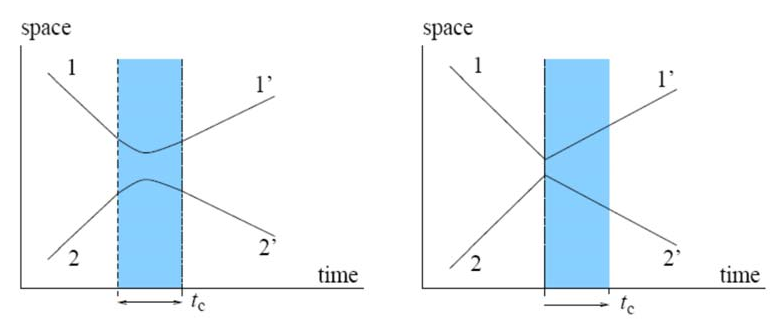
\includegraphics[width=.85\textwidth]{pics/hardpart_comp}
  \captionof{figure}{Comparison of soft particle (left) and hard particle (right) collision.}
  \label{fig:comp_tcmolde}
\end{figure}



\vspace{0.2cm}
If we try to calculate the total time that the ball takes to come at rest, we have to sum up over infinite events each separated by twice the time that the ball takes to hit the ground, $t_j$ (first the ball has to rise and then it falls). Since the height is directly proportional to the energy, also the height scales with the restitution factor at every bounce.  Due to this, at the $j^{th}$  bounce we will have a damping of the height proportional to  $r^j$. With Newtonian mechanics we can compute the time that the ball needs to cover that distance:



\begin{align*}
t_{tot} &= \sum_{j=1}^\infty {t_j}\\
&= 2 \sqrt{\frac{2 h^{\text{initial}}}{g}}  \sum_{j=1}^{\infty} {\sqrt{r^j}}\\
&= 2\sqrt{\frac{2 h^{\text{initial}}}{g}}\kl{\frac{1}{1-\sqrt{r}}-1}
\end{align*}

%10b -5min

The problem in the method lies in the assumption that the interactions are instantaneous. On the contrary, real collisions have a certain duration. Luding and McNamara \citep{ludingmcnamara} introduced a coefficient of restitution that is dependent of the time elapsed since the last event occurred. If the last collision for one of the event partners is less than $t_{\text{contact}}$, then the coefficient is set to one:
%(BLABLA  both??? fehler in folie 44, da heisst es "both particles") 
\begin{equation}
r^{i,j} =\begin{cases}
  r,  & \text{for } t^{i}>t_{\text{contact}} \text{ or } t^{j}>t_{\text{contact}}\\
  1, & \text{otherwise }.
\end{cases}
\end{equation}

Depending on the materials that one wants to simulate more complex dependencies can be used. If , for example, one has a very dense and viscous material 0 instead of 1 can be used. In this case the particles form clusters and stick together.

Comparing soft potential in molecular dynamics and the event driven hard particles (see Fig. \ref{fig:comp_tcmolde}) we see the main difference. In the first case the collision was discretized, while in event driven we have strict binary collision that are instantaneous. In molecular dynamics the condition is softened and multiple collision may occurr in the same time.
          




















